\section{Axiale Lasermoden}

In diesem Teil beschäftigen wir uns mit den axialen Lasermoden. Dafür verwenden wir ein durchstimmbares konfokales Fabry-Pérot-Interferometer. 
Dazu führt man den Laser möglichst parallel in das Interferometer. Die vom Fabry-Pérot-Interferometer durchgelassene Intensität wird dann von einer 
Photodiode detektiert, verstärkt um einen Faktor 100 und dann grafisch dargestellt. Die Rampenspannung des Interferometers wird dann so eingestellt, 
das man 2 mal den freien Spektralbereich sieht. Dies erkennt man daran, dass man genau zwei mal das gleiche Bild nebeneinander auf dem Oszilloskop sieht. 
Den Abstand der Lasermoden bestimmen wir einfach durch Ablesen am Oszilloskop. Zuvor müssen wir aber herausfinden, wie das Zeitsignal auf der 
x-Achse des Oszilloskops mit der Frequenz zusammenhängt.\\

Dazu nehmen wir zwei mal den selben Peak, aber in zwei nebeneinanderliegenden Darstellungen auf Channel 1 in Abbildung \ref{bild:FreierSpektralbereich}.
Dieser Abstand entspricht dem freien Spektralbereich des Interferometers. Dieser ist bei dem hier verwendeten Gerät 2\,GHz. Man könnte ebenfalls das Triggersignal verwenden, 
aber an den Peaks kann man das Maximum leichter ablesen. Man erhält also den Umrechnungsfaktor 

\begin{equation*}
    m = (152 \pm 7)\,\frac{\mathrm{MHz}}{\mathrm{ms}}
\end{equation*}

für die Umrechnung 

\begin{equation}
    \Delta \nu = m\cdot \Delta t
    \label{eq:Umrechnung}
\end{equation}

von der vom Oszilloskop ausgegebenen Zeitdifferenz in Frequenzen $\nu$.


\begin{figure}[ht]
    \centering
    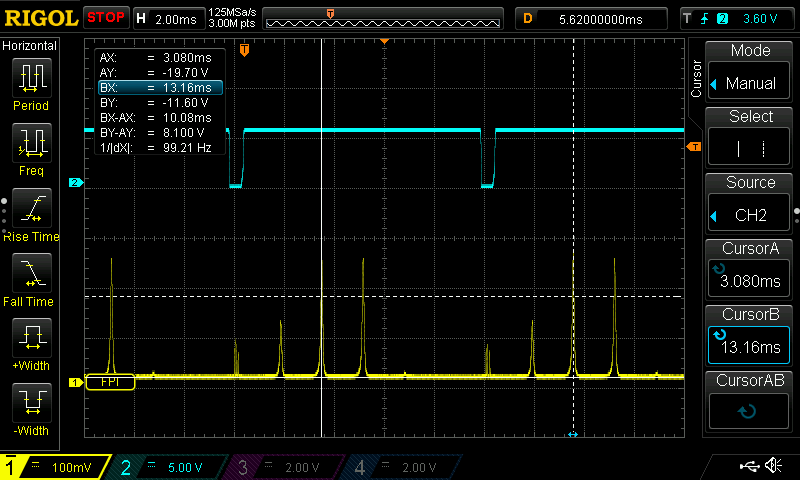
\includegraphics[width = \linewidth]{Bilder/Auswertung/FabryPerotKalibr.png}
    \caption{Longitudinale Lasermoden mit dem Fabry-Pérot aufgenommen. Channel 1 ist das Messsignal und Channel 2 ist des Triggersignal des Interfermoters. Gekennzeichnet sind 
    mit den x-Marker zwei gleich Peaks.}
    \label{bild:FreierSpektralbereich}
\end{figure}


\subsection*{Abstand und Linienbreite Axialer Lasermoden}

Den Abstand der Moden bestimmt man auch grafisch aus Abbildung \ref{bild:AxialModenAbstand}. Aus diesem erhält man 
\begin{equation*}
    \Delta t = (1,660 \pm 0,086)\,\mathrm{ms}
\end{equation*}
und mit der Umrechnung aus Gleichung \ref{eq:Umrechnung} erhalt man 

\begin{equation}
    \textcolor{red}{\delta \nu = (252 \pm 17)\,\mathrm{MHz}}
    \label{eq:Modenabstand}
\end{equation}

den Abstand zweier longitudinaler Lasermoden. Die Unsicherheit wird hierbei aus geschätzter Ableseunsicherheit und
der Unsicherheit der Kalibrierung  mittels Fehlerfortpflanzung berechnet. Auf selbe Weise wird 

\begin{equation}
    \textcolor{red}{\Delta \nu_{multi} = (13,3 \pm 1,5)\,\mathrm{MHz}}
\end{equation}

auch die Linienbreite (FWHM) aus Abbildung \ref{bild:Lininebreite} bestimmt. Gleiches tun wir auch für die einzelne Mode
aus Abbildung \ref{bild:LininebreiteSingle}. Damit erhalten wir die Werte, welche in Tabelle \ref{tab:Linienbreite} dargestellt sind.

\begin{table}
    \centering
 
    \begin{tabular}{lcr}
        \toprule
        Messgröße & Symbol & Wert in MHz\\
        \midrule
        Freier spektraler Bereich& $\Delta \nu_{FSB}$ & 2000\\
        Modenabstand& $\delta\nu$& $252 \pm 17$\\
        FWHM (multi-mode)& $\Delta\nu_{multi}$&$13,3 \pm 1,5$\\
        FWHM (single)& $\Delta\nu_{multi}$&$16,7 \pm 2,6$\\
        \bottomrule        
    \end{tabular}
  
    \caption{Freier spektraler Bereich, Modenabstand, Halbwertsbreite des He-Ne-Laser und dem dazugehörendem 
    konfokalem Fabry-Pérot-Interferometer}
    \label{tab:Linienbreite}
\end{table}


\subsection*{Verstärkungsprofil}

Um das Verstärkungsprofil zu bestimmen haben wir das Oszilloskop auf einen Modus gestellt, bei dem es alle Spuren 
überlagert. Dies haben wir getan und haben den Tisch mit leichten Erschütterungen zum vibrieren gebracht.
Dies führte zu dem benötigten Längenänderungen im Resonator, sodass die Peaks der Moden gewackelt haben.
Somit kann man, wenn man mit den Linien wackelt, ein ungefähres Bild bekommen, wie das Verstärkungsprofil
des Verstärkers aussieht. Das Ergebnis ist in Abbildung \ref{bild:Verstaerkung} sichtbar.

\begin{figure}[h]
    \centering
    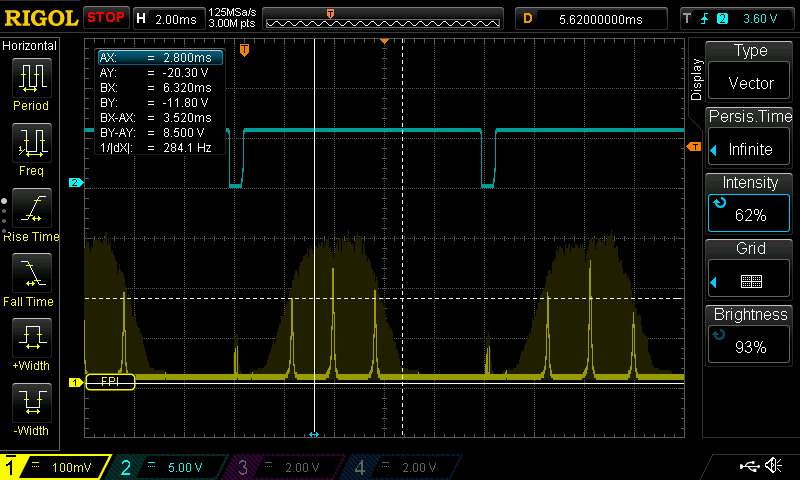
\includegraphics[width = \linewidth]{Bilder/Auswertung/FabryPerotVerst.png}
    \caption{Longitudinale Lasermoden mit dem Fabry-Pérot aufgenommen. Durch Erschütterung wurde das Verstärkungsprofil sichtbar gemacht.}
    \label{bild:Verstaerkung}
\end{figure}

Von diesem schätzen wir die Halbwertsbreite ab, soweit das geht. Die Halbwertsbreite 

\begin{equation}
    \textcolor{red}{\Delta \nu_{Verstärkungsprofil} = 532\pm80\;\mathrm{MHz}}
\end{equation}

hat einen relativ großen Fehler, da man die Spitze des Verstärkungsprofils nicht genau sehen kann und daher abschätzen muss.
Dies ist auch sinnvoll, da die Breite des Verstärkungsprofils mehrmals den Modenabstand beinhalten sollte.


\subsection*{Finesse und Auflösungsvermögen}

Die Finesse und das Auflösungsvermögen sind zwei Größen, die zur Charakterisierung des Resonators nützlich sind. Die Finesse ist dabei
definiert über das Verhältnis 
\begin{align}
    \mathcal{F} = \frac{\delta \nu_{FSR}}{\Delta\nu} \qquad s_{\mathcal{F}} = \sqrt{(\frac{s_{\Delta \nu}*\delta \nu_{FSR}}{\Delta\nu^2})^2+(\frac{s_{\delta\nu}}{\Delta \nu})^2}
\end{align}
 des freien Spektralbereichs zur Linienbreite. Die Auflösung 

 \begin{align}
     A = \frac{\nu}{\Delta\nu} = \frac{c}{\lambda\Delta\nu} \qquad s_A = A\sqrt{()\frac{s_{\Delta\nu}}{\Delta\nu})^2} = A\frac{s_{\Delta\nu}}{\Delta\nu}
 \end{align}
 
 ist hingegen das Verhältnis der Linienbreite zur Frequenz der Spektrallinie. Dabei wurde die Frequenz in
 die Lichtgeschwindigkeit 